\renewcommand{\theequation}{\theenumi}
\begin{enumerate}[label=\thesubsection.\arabic*.,ref=\thesubsection.\theenumi]
\numberwithin{equation}{enumi}

\item \solution A circle passing through three non-collinear points is the circumcircle and the center is the circumcenter.\\
\begin{align}
\vec{O} &= \frac{A\sin{\angle 2A} + B\sin{\angle 2B} + C\sin{\angle 2C}}{\sin{\angle 2A} + \sin{\angle 2B} + \sin{\angle 2C}}\nonumber
\end{align}\\

\item To find the angles:
\begin{align}
\cos{\angle A} &= \frac{ \brak{\vec{C}-\vec{A}}^T \brak{\vec{B}-\vec{A}}}{\| \vec{C}-\vec{A} \|\ \| \vec{B}-\vec{A} \|} \\
\cos{\angle B} &= \frac{ \brak{\vec{A}-\vec{B}}^T \brak{\vec{C}-\vec{B}}}{\| \vec{A}-\vec{B} \|\ \| \vec{C}-\vec{B} \|} \\
\cos{\angle C} &= \frac{ \brak{\vec{A}-\vec{C}}^T \brak{\vec{B}-\vec{C}}}{\| \vec{A}-\vec{C} \|\ \| \vec{B}-\vec{C} \|} 
\end{align}

\item Substituting the give values:
\begin{align}
\therefore \vec{O} &= \myvec{3\\-2}
\end{align}


\item \begin{figure}[!ht]
\centering
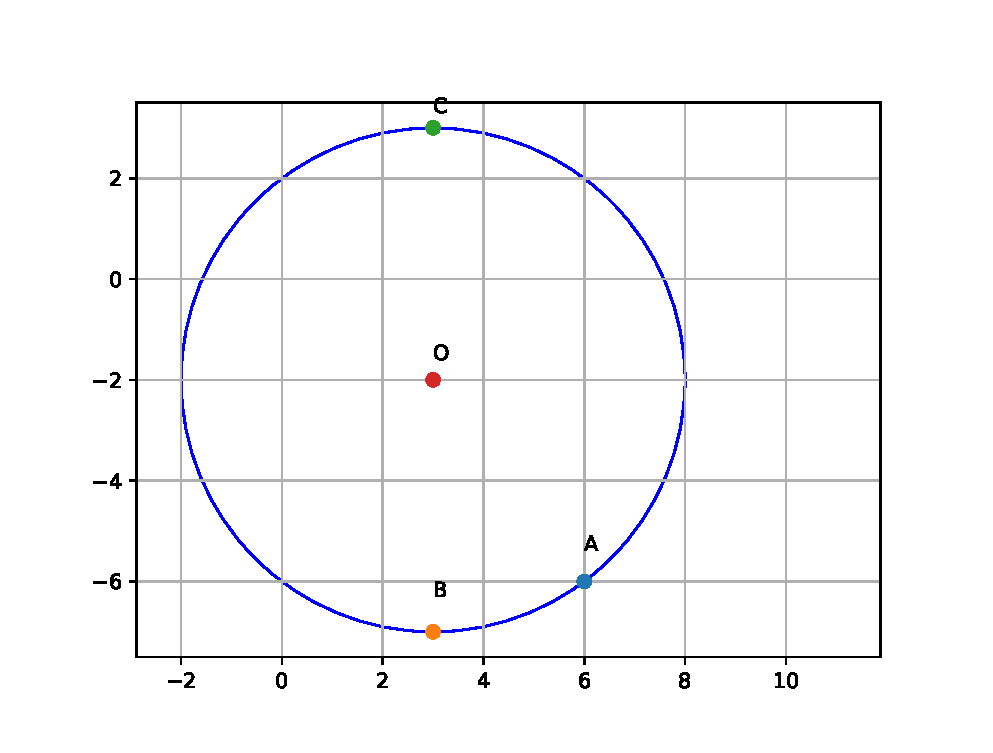
\includegraphics[width=\columnwidth]{./figs/circle_ex/circumcircle.eps}
\caption{Circumcircle generated using python}
\label{fig:Circumcircle2_circle_ex}
\end{figure} 

The following Python code generates Fig. \ref{fig:Circumcircle2_circle_ex}

\begin{lstlisting}
codes/circle_ex/circumcircle.py
\end{lstlisting}
\end{enumerate}



